\documentclass{bioinfo}
\copyrightyear{2015} \pubyear{2015}

\access{Advance Access Publication Date: Day Month Year}
\appnotes{Manuscript Category}\usepackage{tikz}
\usetikzlibrary{arrows}
\usetikzlibrary{patterns}
\usetikzlibrary{decorations.pathreplacing}
\usepackage{multirow}
\usepackage{mathrsfs}
\usepackage{here}
\usetikzlibrary{automata,positioning}

\begin{document}
\firstpage{1}

\subtitle{Genome analysis}

\title[short Title]{Unnamed : A new method for the production of synthetic long reads}
\author[Sample \textit{et~al}.]{Pierre Morisse\,$^{\text{\sfb 1,}*}$, Thierry Lecroq\,$^{\text{\sfb 1}}$ and Arnaud Lefebvre\,$^{\text{\sfb 1}}$}
\address{$^{\text{\sf 1}}$ Computer Science Department, LITIS Laboratory, University of Rouen, 76000 Rouen \\}

\corresp{$^\ast$To whom correspondence should be addressed.}

\history{Received on XXXXX; revised on XXXXX; accepted on XXXXX}

\editor{Associate Editor: XXXXXXX}

\abstract{\textbf{Motivation:} Since a few years, long reads sequencing technologies are being developed and allow the solving of assembly problems
for large and complex genomes that were, until then, unsolvable with the use of short reads sequencing technologies alone. However, despite the fact they can reach lengths of tens of kpb, these long reads are also very noisy, and can reach an error rate as high as 30\%. The vast majority of these error being insertions and deletions, classical error correction tools developed for short reads, which mainly focus on mismatches error, are not effective for correcting long reads. NaS, developed in 2015, uses these noisy long reads as templates to produce assemblies of related accurate short reads, thus yielding accurate synthetic long reads as corrections for the templates.  \\
\textbf{Results:} We present Unnamed, a new method for the production of synthetic long reads, that gets rid of the bottleneck step from NaS. Our experiments show that, while producing comparable results both in terms of length and accuracy of the synthetic long reads, Unnamed is several orders of magnitude faster than NaS. \\
\textbf{Availability:} Unnamed is freely available, under open-source licence at (github) \\
\textbf{Contact:} \href{pierre.morisse2@univ-rouen.fr}{pierre.morisse2@univ-rouen.fr}\\
\textbf{Supplementary information:} Supplementary data are available at \textit{Bioinformatics} online.}

\maketitle

\section{Introduction}
\label{sec:introduction}

Since a few years, long reads sequencing technologies are being developed, and allow the solving of assembly problems for large and complex
genomes that were impossible with the use of short reads sequencing technologies alone. The two major actors of these long reads sequencing technologies are
Pacific Biosciences and Oxford Nanopore, which, with the release of the MinION device, allowed a low-cost and easy long reads sequencing. \\
\indent However, even though long reads can reach lengths of tens of kbp, they also reach a very high error rate of around 15\% for Pacific Biosciences, and up to 30\% for Oxford Nanopore, the vast majority of these errors being insertions and deletions. Correcting these long reads before using them to solve assembly problems is therefore mandatory. Many methods are available for short reads correction, but these methods are not applicable to the long reads, on the one hand because of their much higher error rate, and on the other because most of the error correction tools for short reads focus on substitution errors, the dominant error type in Illumina data, whereas insertions and deletions are more common in long reads. \\
\indent Recently, several methods for long reads correction have been developed. These methods can be divided into two main categories: either
the long reads are selfcorrected by aligning them against each other (HGAP (\cite{Chin2013}), Sprai (CITE) PBcR (CITE, LoRMA), not that many others), or either a hybrid strategy is adopted, in which the long reads are corrected with the help of accurate short reads (LSC (\cite{Au2012}), CoLoRMap (\cite{Haghshenas2016}), LSCPLus (\cite{Hu2016}), loads of others). De Bruijn graphs based methods, where the long reads are mapped on the graph, and erroneous regions corrected by traversing its paths, also seem to develop, in the hybrid case (LoRDEC (\cite{Salmela2014}), Jabba (\cite{Miclotte2016}), as well as in the non-hybrid case (LoRMA (\cite{Salmela2016})). \\
\indent NaS (\cite{Madoui2015}), however, instead of directly correcting the long reads, uses them as templates to produce synthetic long reads from an assembly of short reads. The short reads are first mapped on the long reads, and then against each other, in order to obtain a subset of related short
reads for each template. A synthetic long read is thus obtained and used as the correction of a given template by assembling the subset of short reads
associated to it. A complete overview of NaS is given Section \ref{sec:NaSO}. \\
\indent In this paper, we present a new method to produce synthetic long reads, that gets rid of the time consuming step of aligning all
the short reads against each other. Instead, we focus on a seed-and-extend approach where we extend and link together the seeds, found by mapping
the short reads on the long reads, with perfectly overlapping $k$-mers from the short reads, found with the help of PgSA (\cite{Kowalski2015}). \\
\indent Our experiments show that, while producing comparable results both in terms of length and accuracy of the synthetic long reads, our method is several orders of magnitude faster than NaS. 


\section{PgSA Overview}
\label{sec:PgSAO}

PgSA, along with GkA (\cite{Philippe2011}) and CGkA (\cite{Niko2013}) are data structures that allow the indexing of a set of reads, in order
to answer the following queries, for a given string $f$ :

\begin{enumerate}
	\item In which reads does $f$ occur?
	\item In how many reads does $f$ occur?
	\item What are the occurrence positions of $f$ ?
	\item What is the number of occurrences of $f$ ?
	\item In which reads does $f$ occur only once?
	\item In how many reads does $f$ occur only once?
	\item What are the occurrence positions of $f$ in the reads where it occurs only once?
\end{enumerate}

In these queries, $f$ can be given either as a sequence of DNA symbols, or as a couple of numbers, representing respectively a read ID, and the
start position of $f$ in that read. \\
\indent As previously mentioned, in order to answer these queries, an index of the reads has to be built. To do so, PgSA first computes the overlaps
between the reads, and merges the reads that do overlap, thus obtaining a pseudogenome, shorter than the naive concatenation of the whole read set. 
Then, an auxiliary array is built to allow the retrieval of the reads from the original set in the pseudogenome. Each record of this array  
associates a read ID in the original reads set to a read offset in the pseudogenome, and contains a flag data that brings complementary information about
the said read and that will be used to handle the requests. \\
\indent As the reads are overlapped during the pseudogenome computation, and the auxiliary array doesn't record any information about their lengths, PgSA will only allow the indexing and querying of a set of reads of same length. However, unlike its peers GkA and CGkA, PgSA doesn't set 
the length of $f$ at compilation time, and thus supports querying for multiple lengths of $f$ without any need to recompute the index, which is why
we chose this data structure over the two others. 


\section{NaS Overview}
\label{sec:NaSO}

NaS is a hybrid method for the error correction of long reads. Unlike other methods, instead of directly correcting the long reads, it rather uses them as
templates. Short reads are mapped both on these templates long reads and against each other in order to gather different subsets of short reads, each 
related to one given template. Once a subset of short reads is obtained, contained short reads are assembled and the produced contig is used as a correction for the related template. More precisely, a synthetic long read is produced as follows: \\
\indent First, the short reads are aligned on the template long read using BLAT (\cite{Kent2002}) (untrue, blat is used for fast mode, and last for sensitive mode, although the NaS paper only mentions blat), in order to find seeds, which are short reads that correctly align with the template. Then, once these seeds are found, all the short reads are aligned against each other, and similar reads are recruited,
with the help of Commet (\cite{Maillet2014}). Finally, the obtained subset of short reads is assembled using Newbler (CITE), and a contig is produced,
and used as the correction of the initial template long read. \\ 
\indent Usually, a single contig is produced, but in repeated regions, a few bad reads can be recruited and therefore yield erroneous contigs 
that must not be associated with the template. To address this issue, and produce a single contig, NaS explicitly builds the contig-graph, 
weighted with the seeds coverage of the contigs. Once the graph is built, the path with the highest total weight is chosen with the Floyd-Warshall
algorithm, and contigs along that path are assembled to generate the final synthetic long read. Finally, the consistency of the synthetic read is checked
by aligning initial short reads and detecting gap of coverage. \\
\indent The reads recruitment is the most important(?) step of the method, as it allows to retrieve short reads corresponding to low quality
regions of the template long read. However, this step is also the bottleneck of the whole NaS pipeline, as it is responsible for 70\% of the
total runtime on average. \\
\indent NaS is able to generate synthetic long reads up to 60kbp, that align entirely to the reference genome with no error, and that span
repetitive regions. On average, the accuracy of the synthetic long reads produced by NaS reaches 99.97\%, without any significant length drop
compared to the input long reads.

\section{Our method}
\label{sec:OMO}

Our method, like NaS, aims to use erroneous long reads as templates, and produce synthetic long reads from an assembly of short reads related to
the templates. However, our main objective is to get rid of the time consuming step of reads recruiting, that requires the mapping of all the short reads
against each other. To do so, we focus on a seed-and-extend approach, where seeds are extended and linked together with perfectly overlapping $k$-mers from the short reads, found with the help of PgSA. The workflow of our method is summarized Figure \ref{OMWorkflow}, and its four main steps are described below. \\

\begin{figure*}
	\centering
	\resizebox{0.75\textwidth}{!}{
		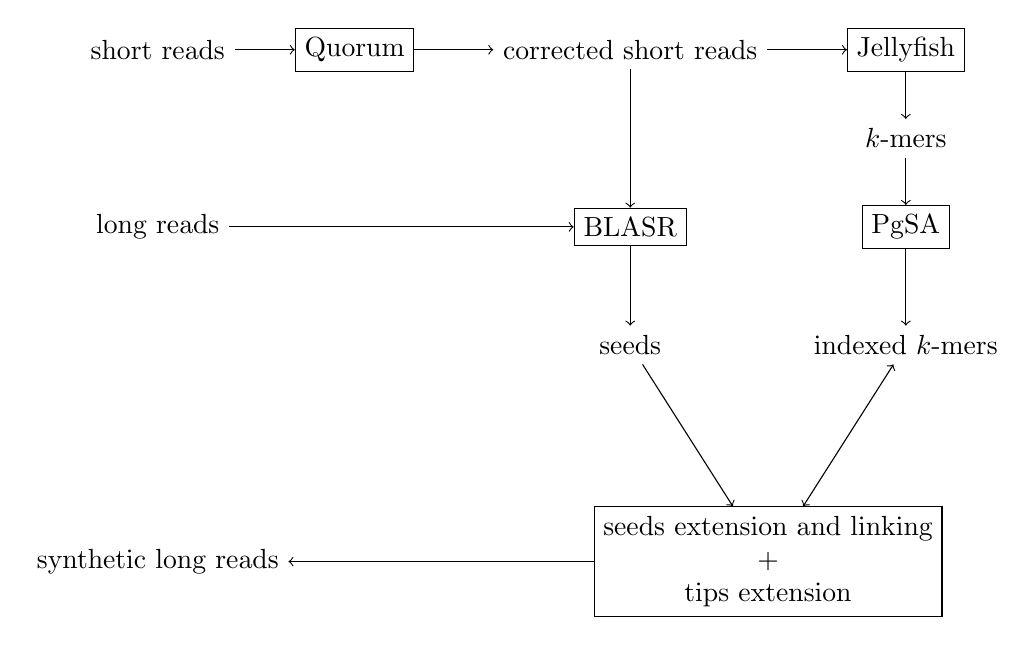
\begin{tikzpicture}
			\node (SR) at (0,0) {short reads};
			\node[draw, rectangle] (Qu) at (2.5,0) {Quorum};
			\draw [->] (SR) -- (Qu);
			\node (CSR) at (6,0) {corrected short reads};
			\draw [->] (Qu) -- (CSR);
			\node[draw, rectangle] (Jel) at (9.5,0) {Jellyfish};
			\draw [->] (CSR) -- (Jel);
			\node (kmers) at (9.5,-1.125) {$k$-mers};
			\draw [->] (Jel) -- (kmers);
			\node[draw, rectangle] (PgSA) at (9.5,-2.25) {PgSA};
			\draw [->] (kmers) -- (PgSA);
			\node (IK) at (9.5,-3.75) {indexed $k$-mers};
			\draw [->] (PgSA) -- (IK);			
			\node[draw, rectangle] (BLASR) at (6,-2.25) {BLASR};
			\node (LR) at (0,-2.25) {long reads};
			\draw [->] (LR) -- (BLASR);
			\draw [->] (CSR) -- (BLASR);
			\node (seeds) at (6,-3.75) {seeds};
			\draw [->] (BLASR) -- (seeds);
			\node[draw, rectangle, align=center] (Link) at (7.75,-6.5) {seeds extension and linking \\ + \\ tips extension};
			\draw [->] (seeds) -- (Link);
			\draw [<->] (IK) -- (Link);
			\node (SLR) at (0,-6.5) {synthetic long reads};
			\draw [->] (Link) -- (SLR);
		\end{tikzpicture}
	}
	\caption{Our method's workflow. First, the short reads are corrected in order to get rid of as much sequencing errors as possible. Then,
	all the $k$-mers from the corrected short reads (and from their reverse complements) are obtained with Jellyfish, and indexed with PgSA.
	Short reads are aligned on long reads with BLASR to find seeds, and the indexed $k$-mers are queried to extend and link together the found
	seeds. Finally, the sequences obtained from the seeds linkage are extended in both directions to reach the initial templates borders, 
	and the synthetic long reads	are output. \label{OMWorkflow}}
\end{figure*}

\subsection{Short reads correction and indexing}

Even though short reads are very accurate prior to any correction, as we seek to use their $k$-mers to compute perfect overlaps and extend the seeds, we need to get rid of as much sequencing errors as we can in this data. We thus correct the short reads with the help of Quorum (\cite{Marcais2015}), which is able to provide a good raise of the accuracy in very little time. Once corrected, the $k$-mers from the short reads and from their reverse complements are extracted with Jellyfish (\cite{Marcais2011}), and indexed with PgSA, before being queried to extend and link the seeds together during the following steps.

\subsection{Seeds retrieving and merging}

Like with NaS, the seeds are found by mapping the corrected short reads on the template long reads. This is done with the help of BLASR (\cite{Chaisson2012}), an alignment tool specifically designed to align long reads dominated by insertion and deletion errors. Then, for each template, two phases of analyze and merging are applied to the associated seeds. First, if the mapping positions of a given couple of seeds imply that they overlap on the template over a sufficient length, their assumed overlapping sequences are compared, and the two seeds are merged accordingly. If the mapping positions indicate the two seeds do overlap on the template, but not over a sufficient length, or if the assumed overlapping sequences do no coincide, then, only the seed with the best alignment score is kept. Then, once seeds having overlapping mapping positions have been merged or filtered out, sequences overlaps between consecutive seeds are computed. Like in the previous step, if a given seed overlaps the following one over a sufficient length, the two seeds are merged.

\subsection{Seeds linking}
Once seeds have been found and merged for each template, our method attempts to link together every couple of seeds, by extending the rightmost $k$-mer of the left seed with perfectly overlapping $k$-mers from the short reads, until the leftmost $k$-mer of the right seed is reached. To do so, PgSA's third request, that gives the occurrences positions of a given string, is looped over to find overlaps of length $k - 1$ between the currently 
considered $k$-mer and the other $k$-mers from the set of short reads. When such an overlap is found, the current $k$-mer is extended
with the non-overlapping bases of the new found one, which is then considered for the next extension. If no overlap of length $k - 1$ is found, then the length is decreased and overlaps are searched again, as PgSA allows requesting for strings of variable lengths. Overlap length thus keeps on decreasing until an overlap is found, or until the minimum length, fixed as $k / 2$ is reached. \\
\indent When requesting PgSA to find overlapping $k$-mers, it is also possible to find multiple $k$-mers that perfectly overlap the currently considered $k$-mer. In such cases, all possible extensions are checked with the use of backtracking, to find the one that will allow correct linking of the two seeds. However, to avoid long runtimes and intensive computations, a threshold on the maximum number of backtracks is set. If this threshold, or the previously defined minimum overlap length, is reached and no path has been found to link the two seeds, then the linking is given up, a new linking is computed for the next seeds couple, and a fragmented synthetic long read is produced.

\subsection{Tips extension}
Finally, it is obvious that seeds don't always map right at the beginning and until the end of the templates. Thus, in order to get as close as possible to the original templates' lengths, once all the seeds have been linked, we keep extending the so produced synthetic long read, on the left of the leftmost seed, and on the right of the rightmost seed, until we reach the template's borders, or an ambiguity. This happens when multiple $k$-mers perfectly
overlap the currently considered $k$-mer, and that its extension is therefore possible with every of these different $k$-mers. As we have no clue as to which one to chose and continue the extension with, nor precise destination, unlike when we attempt to link two seeds, the extension is simply stopped when such a situation occurs. 


\section{Results and discussion}
\label{sec:results}

We compare the quality of our synthetic long reads with those produced by NaS, and also with the corrected long reads produced by others state-of-the-art
hybrid correction methods, namely LoRDEC and CoLoRMap. We compare the results both in terms of mapping quality of the produced reads on the reference genome, and of quality of the assembly that was generated from the reads.

\subsection{Datasets}

As we mainly seek to compare our results with NaS, we use same data to allow a better comparison. This data is composed of both long MinION and short Illumina reads for three different genomes: \emph{Acinetobacter baylyi}, \emph{Escherichia coli}, and \emph{Saccharomyces cerevisae}. Details are given Table \ref{tabdata}.

\begin{table*}[t]
	\resizebox{\textwidth}{!}{
	\begin{tabular}{|c|cccc|ccc|ccc|}
		\hline
		\multirow{2}{*}{\textbf{Dataset}} & \multicolumn{4}{c|}{\textbf{Reference genome}} & \multicolumn{3}{c|}{\textbf{MinION data}} & 
		\multicolumn{3}{c|}{\textbf{Illumina data}} \\
		& \textbf{Name} & \textbf{Strain} & \textbf{Reference sequence} & \textbf{Genome size} & \textbf{Number of reads} & \textbf{Average length} &
		\textbf{Coverage} & \textbf{Number of reads} & \textbf{Read length} & \textbf{Coverage}\\
 		\hline
		ADP1 & \emph{Acinetobacter baylyi} & ADP1 & CR543861 & 3.6 Mbp & 89,011 & 4,285 & 103x & 900,000 & 250 & 50x \\
		\hline
		Ecoli & \emph{Escherichia coli} & K-12 substr. MG1655 & NC\_000913 & 4.6 Mbp & 22,270 & 5,999 & 29x & 775,500 & 300 & 50x \\
		\hline
		Yeast & \emph{Saccharomyces cerevisae} & W303 & lala & 12 Mbp & 205,923 & 5,698 & 98x & 2,500,000 & 250 & 50x \\
		\hline
	\end{tabular}
	} \\
	\caption{Description of the datasets used in our experiments. \label{tabdata} Both MinION and Illumina data are available from the Genoscope website: 
	http://www.genoscope.cns.fr/externe/nas/datasets.html TODO : MinION coverage \`a revoir}
\end{table*}

\begin{table*}[t!]
	\resizebox{\textwidth}{!}{
	\begin{tabular}{|c|c|c|c|c|c|c|c|c|c|}
		\hline
		\textbf{Dataset} & \textbf{Tool} & \textbf{Number of reads} & \textbf{Average length} & \textbf{Cumulatize size} & 
		\textbf{Number of aligned reads} & \textbf{Average identity} & \textbf{Error free reads} & \textbf{Genome coverage}
		& \textbf{Runtime} \\
		\hline
		\multirow{3}{*}{ADP1} & \textbf{Original} & 70,314 & 2,530 & 177,869,033 & 373 & 3.84 \% & 0 & N.A. & N.A. \\
		& \textbf{NaS (fast)} & 8,219 & 4,514 & 37,099,564 & 8,219 & 99.92 \% & 8,025 & 99.96 \% & TODO \\
		& \textbf{NaS (sensitive)} & 12,053 & 6,338 & 76,388,104 & 12,053 & 99.89 \% & 11,665 & 100 \% & TODO \\
		& \textbf{Our method} & 7,425 (249 fragmented) & 10,250 & 78,739,767 & 7,676 & 99.56 \% & 7,081 & 99.93 \% & TODO \\
		\hline
		\multirow{3}{*}{Yeast} & \textbf{Original} & 158,896 & 5,525 & 877,844,119 & 1,547 & 2,55 \% & 0 & N.A. & N.A. \\
		& \textbf{NaS (fast)} & 44,446 & 5,178 & 230,158,404 & 44,363 & 99.63 \% & 37,607 & 98.01 \% & TODO \\
		& \textbf{NaS (sensitive)} & 56,942 & 6,221 & 354,255,034 & 56,837 & 99,55 \% & 47,122 & 98.68 \% & TODO \\
		& \textbf{Our method} & TODO & TODO & TODO & TODO & TODO & TODO & TODO & TODO \\
		\hline
	\end{tabular}
	}
	\caption{Test on 1D MinION reads \label{tabres1}}
\end{table*}

\begin{table*}[t!]
	\resizebox{\textwidth}{!}{
	\begin{tabular}{|c|c|c|c|c|c|c|c|c|c|}
		\hline
		\textbf{Dataset} & \textbf{Tool} & \textbf{Number of reads} & \textbf{Average length} & \textbf{Cumulatize size} & 
		\textbf{Number of aligned reads} & \textbf{Average identity} & \textbf{Error free reads} & \textbf{Genome coverage}
		& \textbf{Runtime} \\
		\hline
		\multirow{3}{*}{ADP1} & \textbf{Original} & 18,697 & 10,884 & 203,496,742 & 13,636 & 37,07 \% & 0 & N.A. & N.A. \\
		& \textbf{NaS (fast)} & 15,844 & 11,084 & 175,607,625 & 15,844 & 99.78 \% & 14,959 & 100 \% & TODO \\
		& \textbf{NaS (sensitive)} & 16,439 & 11,871 & 195,138,674 & 16,439 & 99.79 \% & 15,525 & 100 \% & TODO \\
		& \textbf{Our method} & 15,575 (984 fragmented) & 10 562 & 178,222,404 & 16,874 & 99.54 \% & 14,791 & 100 \% & TODO \\
		\hline
		\multirow{3}{*}{Ecoli} & \textbf{Original} & 22,270 & 5,999 & 133,607,392 & 21,318 & 39,08 \% & 0 & N.A. & N.A. \\
		& \textbf{NaS (fast)} & 21,818 & 7,926 & 172,918,739 & 21,818 & 99.86 \% & 20,383 & 100 \% & TODO \\
		& \textbf{NaS (sensitive)} & 22,144 & 8,307 & 183,958,832 & 22,144 & 99.86 \% & 20,627 & 100 \% & TODO \\
		& \textbf{Our method} & TODO & TODO & TODO & TODO & TODO & TODO & TODO & TODO \\
		\hline
		\multirow{3}{*}{Yeast} & \textbf{Original} & 47,027 & 6,285 & 295,545,390 & 15,192 & 8,75 \% & 0 & N.A. & N.A. \\
		& \textbf{NaS (fast)} & 27,347 & 7,123 & 196,167,951 & 27,301 & 99.52 \% & 22,181 & 97,82 \% & TODO \\
		& \textbf{NaS (sensitive)} & 28,490 & 7,866 & 224,096,554 & 28,451 & 99.47 \% & 22,693 & 98,61 \% & TODO \\
		& \textbf{Our method} & TODO & TODO & TODO & TODO & TODO & TODO & TODO & TODO \\
		\hline
	\end{tabular}
	}
	\caption{Test on 2D MinION reads \label{tabres2}}
\end{table*}

\begin{table*}[t!]
	\resizebox{\textwidth}{!}{
	\begin{tabular}{|c|c|c|c|c|c|c|}
		\hline
		\textbf{Dataset} & \textbf{Tool} & \textbf{Number of reads} & \textbf{Expected contigs} & \textbf{Number of contigs} & \textbf{Genome coverage} & \textbf{Identity} \\
		\hline
		\multirow{3}{*}{ADP1} & \textbf{Original} & 89,011 & N.A. & N.A. & N.A. & N.A. \\
		& \textbf{NaS (fast)} & 24,063 & 1 & 1 & 100 \% & 99.98 \% \\
		& \textbf{NaS (sensitive)} & 28,492 & 1 & 1 & 100 \% & 99.99 \% \\
		& \textbf{Our method} & TODO & 1 & TODO & TODO & TODO \\
		\hline
		\multirow{3}{*}{Ecoli} & \textbf{Original} & 22,270 & N.A. & N.A. & N.A. & N.A. \\
		& \textbf{NaS (fast)} & 21,818 & 1 & 1 & 99,90 \% & 99.99 \% \\
		& \textbf{NaS (sensitive)} & 22,144 & 1 & 1 & 100 \% & 99.99 \% \\
		& \textbf{Our method} & TODO & 1 & TODO & TODO & TODO \\
		\hline
		\multirow{3}{*}{Yeast} & \textbf{Original} & 205,923 & N.A. & N.A. & N.A. & N.A. \\
		& \textbf{NaS (fast)} & 71,793 & 30 & 124 & 97.27 \% & 99.78 \% \\
		& \textbf{NaS (sensitive)} & 85,432 & 30 & 120 & 97.04 \% & 99.79 \% \\
		& \textbf{Our method} & TODO & 30 & TODO & TODO & TODO \\
		\hline
	\end{tabular}
	}
	\caption{Assembly results \label{tabres3}}
\end{table*}

\subsection{Mapping quality}

We recall that Oxford Nanopore technologies can yield both 1 direction and 2 directions, longer and more accurate, reads. We correct both types of reads separately, to be able to better analyze the results, and compare the different correction methods more in depth. Results on the 1D reads are given Table \ref{tabres1}, and results on the 2D reads are given Table \ref{tabres2}. The raw long reads were aligned using Last (\cite{Kielbasa2011}), and the corrected long reads were aligned using BWA (\cite{Li2009}). We discuss and analyze the results below. \\
\indent We notice that the synthetic long reads produced from 1D templates by our method are longer than those produced by NaS, both in fast or sensitive mode. This is likely caused by the last extension step, when Unnamed extends the tips of the synthetic long reads as much as possible, until the borders of the template or an ambiguity is reached. As a result, the cumulative size of these reads is also greater than the one obtained with NaS. \\
\indent With 2D templates, however, synthetic long reads produced by NaS are longer than those produced by our method, even in sensitive mode. We can suppose this is due to the fact that fragmented reads are present in greater proportion on the synthetic long reads produced from 2D reads (6 \% of the synthetic reads produced from 2D templates are fragmented, whereas only 3 \% of those produced from 1D templates are), and that therefore, they do induce a drop of the average length. \\
\indent Synthetic long reads produced by our method tend to have a lower identity than those produced by NaS. This is probably caused by ??? \\
\indent We also notice that Unnamed produces less synthetic long reads that NaS, which is due to the parameters used when mapping short reads on long reads
to discover seeds. We indeed set the bestn parameter from BLASR to 30, meaning that for each short read, only the best 30 mapping positions are output. Raising the bestn parameter therefore allows to output more mapping positions on more different template long reads, and thus to produce more synthetic long reads, but also causes a raise in the runtime of the mapping step.

\subsection{Assembly quality}
	
All the corrected long reads datasets were assembled using Canu (\cite{Koren2016}), without the correction step. Results are given Table \ref{tabres3} and discussed below. \\
\indent Synthetic long reads produced by NaS were able to be assembled into a single contig for both \emph{Acinetobacter baylyi} and \emph{Escherichia coli}, by using Canu with default parameters. However, those produced by our method needed a little tuning of Canu parameters (OvlMerSize=17, MhapMerSize=17, OvlMerDistinct=0.995, OvlMerTotal=0.995, correctedErrorRate=0.10) to be able to generate a single contig. This need to tune the parameters is likely due to the production of fragmented synthetic long reads, when Unnamed is unable to link two seeds, causing a drop of length and a loss of information in the gaps that couldn't be resolved. For \emph{Saccharomyces cerevisae}, both methods failed to assemble the long reads into the expected number of contigs, however, ??? slightly outperformed ??? We also notice that the contigs produced by our method tend to cover the reference genome a bit less than NaS for the three studied genomes, and that their identity is also slightly lower. However, it is likely that by finding a better tuning of the parameters, both for the correction step of our method and for the Canu assembly, our method will be able to better cover the reference genome, with a better identity. 
		

\section{Conclusions}
\label{sec:conclusions}

We developed a new hybrid strategy for the correction of long reads, that, like NaS, focuses on the production of synthetic long reads, by an assembly of short reads related to a given template, rather that on the direct correction of the input long reads. Also, rather than aligning the short reads
against each other in a recruiting step, and then assembling the obtained subset of reads with already existing tools, like NaS, we focused on a brand new idea of directly assembling $k$-mers from the short reads data. For this aim, we used as seeds short reads that aligned perfectly on the input long reads, used as templates, and linked them together with perfectly overlapping $k$-mers from the short reads, found with the help of PgSA, a data structure allowing to index and query a set of reads or $k$-mers. \\
\indent We tested this new method and compared it with NaS on three different genomes, namely \emph{Acinetobacter baylyi}, \emph{Escherichia coli}, and \emph{Saccharomyces cerevisae}. On these three genomes, Unnamed yielded results that compared well with NaS, while being several orders of magnitude faster. \\
\indent The development of this method showed that, when having templates and anchor points (in this case, our seeds), PgSA and related data structures could prove useful to product an assembly from $k$-mers, or even from complete reads. It could be interesting to focus more on this idea, and try to see if it could produce a proper assembly tool, for short reads as well as for long reads. 


\section*{Acknowledgements}

Stuff


\section*{Funding}

Stuff

\bibliographystyle{natbib}
%\bibliographystyle{achemnat}
%\bibliographystyle{plainnat}
%\bibliographystyle{abbrv}
%\bibliographystyle{bioinformatics}
%
%\bibliographystyle{plain}
%
%\bibliography{Document}


%\bibliographystyle{abbrv}
\bibliography{../../../Bibliographies/library}
\end{document}
